\section{Fundamentals of Particle Image Velocimetry}

Particle Image Velocimetry, or PIV, is a class of methods employed by 
experimental fluid mechanics to measure instantaneous vector velocity fields by 
measuring the displacements of small visible particles which follow the motion 
of the fluid \cite{adrian2011}. Figure \ref{fig:quiver_example} shows a typical 
resulting vector field from measurements of a vortical flow. Each of these 
two-dimensional vectors was measured simultaneously in a thin sheet of fluid. 
The velocity of the fluid is sensed by acquiring images of well entrained 
particles at precise times and measuring the displacement of those particles. 
This technique can be used to study flows in gases and liquids, and is derived 
from techniques originally developed to measure mechanical 
deformations and stresses in solids.

\begin{figure}[H]
	\centering
	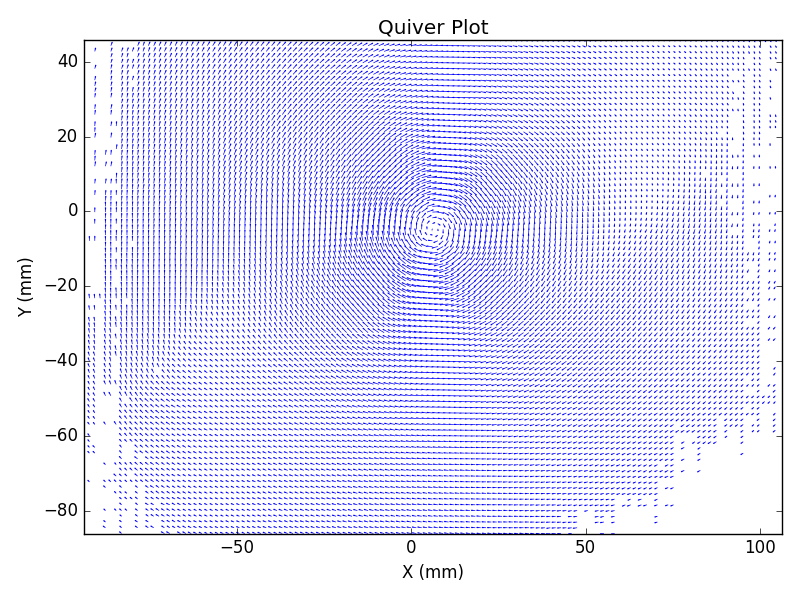
\includegraphics[width=5in]{figs/example_vortex_figs/example_quiver}
	\caption{Velocity vector field of a vortical flow structure as produced by 
	PIV.}
	\label{fig:quiver_example}
\end{figure}

 
\subsection{The Case for PIV}

Unlike other flow measurement techniques, PIV is a non-invasive method to 
directly measure time and displacement, and thus velocity.

\subsection{Cameras and Lighting}

\subsection{Particles}

\subsubsection{Particle Dynamics} 

\subsubsection{Error Due to Slip}

\subsubsection{Seeding Particles for PIV}

\subsection{Image processing}

\subsection{Interrogation}

\subsection{Measurement of Fluid Flow}

\subsection{PIV in Three Dimensions}

\subsection{Practical PIV Systems}


